\section*{5.1 单变量函数微分}
\addcontentsline{toc}{section}{5.1 单变量函数微分}
\label{sec:5.1}

下面，我们简要回顾单变量函数的微分，这在高中数学中可能已经很熟悉。我们首先从单变量函数 $ y = f(x) $（$ x, y \in \mathbb{R} $）的差商出发，随后利用它来定义导数。

\textbf{定义 5.1}（差商）。 \emph{差商（difference quotient）} ：

\begin{equation}
\frac{\delta y}{\delta x} := \frac{f(x + \delta x) - f(x)}{\delta x}
\tag{5.3}\label{eq:5-3}
\end{equation}

用于计算经过函数 $ f $ 图形上两点的割线斜率。在图~\ref{fig:5-3} 中，这两个点的 $ x $ 坐标分别为 $ x_0 $ 和 $ x_0 + \delta x $。


\begin{figure}[H]
\centering
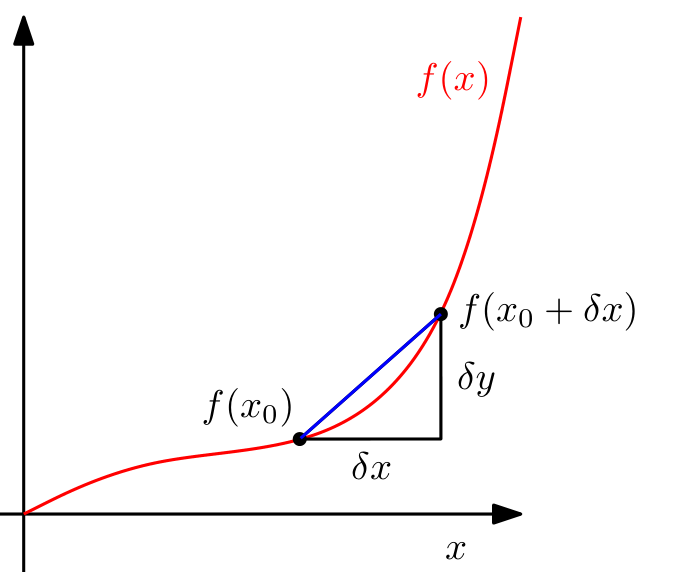
\includegraphics[width=0.92\textwidth,keepaspectratio]{docs/images/Figure5.3.png}
\caption*{\refstepcounter{figcounter}\label{fig:5-3}图~\thefigcounter 函数 f 在 x₀ 与 x₀ + δx 之间的平均倾斜度是通过 f(x₀) 和 f(x₀ + δx) 的割线（蓝色）的斜率，由 δy/δx 给出。}
\end{figure}


如果假定 $ f $ 为线性函数，差商也可以看作是 $ f $ 在 $ x $ 与 $ x + \delta x $ 之间的平均斜率。当 $ \delta x \to 0 $ 时，若 $ f $ 可微，极限即为 $ f $ 在 $ x $ 处的切线斜率。该切线即为 $ f $ 在 $ x $ 处的导数。

\textbf{定义 5.2}（导数）。更正式地，对于 $ h > 0 $，函数 $ f $ 在 $ x $ 处的 \emph{导数（derivative）} 定义为极限：

\begin{equation}
\frac{\mathrm{d}f}{\mathrm{d}x} := \lim_{h \to 0} \frac{f(x + h) - f(x)}{h}
\tag{5.4}\label{eq:5-4}
\end{equation}

此时图~\ref{fig:5-3} 中的割线收敛为切线。函数 $ f $ 的导数指向 $ f $ 最陡上升的方向。

\begin{notebox}
\textbf{例 5.2（多项式的导数）}
\end{notebox}

\begin{notebox}
我们希望计算 $ f(x) = x^n $（$ n \in \mathbb{N} $）的导数。我们可能已经知道结果是 $ n x^{n-1} $，但我们希望利用导数作为差商极限的定义来推导这一结果。
\end{notebox}

\begin{notebox}
利用式~\eqref{eq:5-4} 中导数的定义，我们有：

\begin{equation}
\frac{\mathrm{d}f}{\mathrm{d}x} = \lim_{h \to 0} \frac{f(x + h) - f(x)}{h}
\tag{5.5a}\label{eq:5-5a}
\end{equation}

\begin{equation}
= \lim_{h \to 0} \frac{(x + h)^n - x^n}{h}
\tag{5.5b}\label{eq:5-5b}
\end{equation}

\begin{equation}
= \lim_{h \to 0} \frac{\sum_{i=0}^n \binom{n}{i} x^{n-i} h^i - x^n}{h}
\tag{5.5c}\label{eq:5-5c}
\end{equation}

注意到 $ x^n = \binom{n}{0} x^{n-0} h^0 $。通过从 $ i = 1 $ 开始求和，常数项 $ x^n $ 相互抵消，从而得到：

\begin{equation}
\frac{\mathrm{d}f}{\mathrm{d}x} = \lim_{h \to 0} \frac{\sum_{i=1}^n \binom{n}{i} x^{n-i} h^i}{h}
\tag{5.6a}\label{eq:5-6a}
\end{equation}

\begin{equation}
= \lim_{h \to 0} \sum_{i=1}^n \binom{n}{i} x^{n-i} h^{i-1}
\tag{5.6b}\label{eq:5-6b}
\end{equation}

\begin{equation}
= \lim_{h \to 0} \left[ \binom{n}{1} x^{n-1} + \sum_{i=2}^n \binom{n}{i} x^{n-i} h^{i-1} \right]
\tag{5.6c}\label{eq:5-6c}
\end{equation}

在式~\eqref{eq:5-6c} 中，当 $ h \to 0 $ 时第二项趋向于 0，因此：

\begin{equation}
\frac{\mathrm{d}f}{\mathrm{d}x} = \frac{n!}{1!(n - 1)!} x^{n-1} = n x^{n-1}
\tag{5.6d}\label{eq:5-6d}
\end{equation}
\end{notebox}

\medskip\hrule\medskip

\section*{5.1.1 泰勒级数}
\addcontentsline{toc}{subsection}{5.1.1 泰勒级数}

泰勒级数是将函数 $ f $ 表示为无限项之和的一种形式。这些项由在 $ x_0 $ 处求值的 $ f $ 的各阶导数所决定。

\textbf{定义 5.3}（泰勒多项式）。函数 $ f : \mathbb{R} \to \mathbb{R} $ 在 $ x_0 $ 处的 $ n $ 阶 \emph{泰勒多项式（Taylor polynomial）} 定义为：

\begin{equation}
T_n(x) := \sum_{k=0}^n \frac{f^{(k)}(x_0)}{k!} (x - x_0)^k
\tag{5.7}\label{eq:5-7}
\end{equation}

其中 $ f^{(k)}(x_0) $ 是 $ f $ 在 $ x_0 $ 处的 $ k $ 阶导数（假定其存在），而 $ \frac{f^{(k)}(x_0)}{k!} $ 是多项式的系数。我们对所有 $ t \in \mathbb{R} $ 约定 $ t^0 := 1 $。

\textbf{定义 5.4}（泰勒级数）。对于光滑函数 $ f \in C^\infty $（$ f : \mathbb{R} \to \mathbb{R} $），$ f $ 在 $ x_0 $ 处的 \emph{泰勒级数（Taylor series）} 定义为：

\begin{equation}
T_\infty(x) = \sum_{k=0}^\infty \frac{f^{(k)}(x_0)}{k!} (x - x_0)^k
\tag{5.8}\label{eq:5-8}
\end{equation}

当 $ x_0 = 0 $ 时，我们获得作为泰勒级数特例的 \emph{麦克劳林级数（Maclaurin series）} 。如果 $ f(x) = T_\infty(x) $，则称 $ f $ 是 \emph{解析的（analytic）} 。这里 $ f \in C^\infty $ 表示 $ f $ 是无穷次连续可微的。

\emph{备注} 。一般而言，$ n $ 阶泰勒多项式是对函数的逼近，该函数本身不一定是多项式。泰勒多项式在 $ x_0 $ 的邻域内与 $ f $ 相似。然而，对于次数 $ k \leqslant n $ 的多项式 $ f $，$ n $ 阶泰勒多项式是该多项式的精确表示，因为所有阶数 $ i > k $ 的导数 $ f^{(i)} $ 全为 0。♦

\begin{notebox}
\textbf{例 5.3（泰勒多项式）}
\end{notebox}

\begin{notebox}
考虑多项式：

\begin{equation}
f(x) = x^4
\tag{5.9}\label{eq:5-9}
\end{equation}

我们求在 $ x_0 = 1 $ 处求值的泰勒多项式 $ T_6 $。首先计算各阶导数系数 $ f^{(k)}(1) $（$ k = 0, \ldots, 6 $）：

\begin{equation}
f(1) = 1
\tag{5.10}\label{eq:5-10}
\end{equation}

\begin{equation}
f'(1) = 4
\tag{5.11}\label{eq:5-11}
\end{equation}

\begin{equation}
f''(1) = 12
\tag{5.12}\label{eq:5-12}
\end{equation}

\begin{equation}
f^{(3)}(1) = 24
\tag{5.13}\label{eq:5-13}
\end{equation}

\begin{equation}
f^{(4)}(1) = 24
\tag{5.14}\label{eq:5-14}
\end{equation}

\begin{equation}
f^{(5)}(1) = 0
\tag{5.15}\label{eq:5-15}
\end{equation}

\begin{equation}
f^{(6)}(1) = 0
\tag{5.16}\label{eq:5-16}
\end{equation}

因此，所需的泰勒多项式为：

\begin{equation}
T_6(x) = \sum_{k=0}^6 \frac{f^{(k)}(x_0)}{k!} (x - x_0)^k
\tag{5.17a}\label{eq:5-17a}
\end{equation}

\begin{equation}
= 1 + 4(x - 1) + 6(x - 1)^2 + 4(x - 1)^3 + (x - 1)^4 + 0
\tag{5.17b}\label{eq:5-17b}
\end{equation}

展开并整理各项得到：

\begin{equation}
T_6(x) = (1 - 4 + 6 - 4 + 1) + x(4 - 12 + 12 - 4) + x^2(6 - 12 + 6) + x^3(4 - 4) + x^4
\tag{5.18a}\label{eq:5-18a}
\end{equation}

\begin{equation}
= x^4 = f(x)
\tag{5.18b}\label{eq:5-18b}
\end{equation}

即我们得到了原函数的精确表示。
\end{notebox}


\begin{figure}[H]
\centering
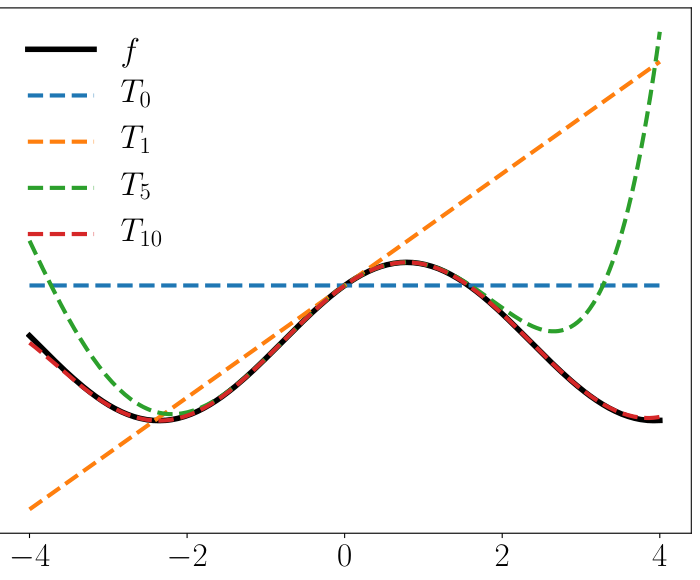
\includegraphics[width=0.92\textwidth,keepaspectratio]{docs/images/Figure5.4.png}
\caption*{\refstepcounter{figcounter}\label{fig:5-4}图~\thefigcounter 泰勒多项式。原函数 f(x) = sin(x) + cos(x)（黑色实线）在 x₀ = 0 处由各阶泰勒多项式（虚线）逼近。高阶泰勒多项式能更好地在更大全局范围内逼近函数 f。T₁₀ 在 [-4, 4] 区间内已经与 f 高度吻合。}
\end{figure}


\begin{notebox}
\textbf{例 5.4（泰勒级数）}
\end{notebox}

\begin{notebox}
考虑图~\ref{fig:5-4} 中给出的函数：

\begin{equation}
f(x) = \sin(x) + \cos(x) \in C^\infty
\tag{5.19}\label{eq:5-19}
\end{equation}

我们求 $ f $ 在 $ x_0 = 0 $ 处的泰勒级数展开（即麦克劳林级数展开）。我们得到以下导数：

\begin{equation}
f(0) = \sin(0) + \cos(0) = 1
\tag{5.20}\label{eq:5-20}
\end{equation}

\begin{equation}
f'(0) = \cos(0) - \sin(0) = 1
\tag{5.21}\label{eq:5-21}
\end{equation}

\begin{equation}
f''(0) = -\sin(0) - \cos(0) = -1
\tag{5.22}\label{eq:5-22}
\end{equation}

\begin{equation}
f^{(3)}(0) = -\cos(0) + \sin(0) = -1
\tag{5.23}\label{eq:5-23}
\end{equation}

\begin{equation}
f^{(4)}(0) = \sin(0) + \cos(0) = f(0) = 1
\tag{5.24}\label{eq:5-24}
\end{equation}

此处存在规律：泰勒级数中的系数仅为 $ \pm 1 $（因为 $ \sin(0) = 0 $），每两个相同符号后切换到另一个符号。此外，$ f^{(k+4)}(0) = f^{(k)}(0) $。
\end{notebox}

\begin{notebox}
因此，$ f $ 在 $ x_0 = 0 $ 处的完整泰勒级数展开为：

\begin{equation}
T_\infty(x) = \sum_{k=0}^\infty \frac{f^{(k)}(x_0)}{k!} (x - x_0)^k
\tag{5.25a}\label{eq:5-25a}
\end{equation}

\begin{equation}
= 1 + x - \frac{1}{2!} x^2 - \frac{1}{3!} x^3 + \frac{1}{4!} x^4 + \frac{1}{5!} x^5 - \cdots
\tag{5.25b}\label{eq:5-25b}
\end{equation}

\begin{equation}
= \left( 1 - \frac{1}{2!} x^2 + \frac{1}{4!} x^4 \mp \cdots \right) + \left( x - \frac{1}{3!} x^3 + \frac{1}{5!} x^5 \mp \cdots \right)
\tag{5.25c}\label{eq:5-25c}
\end{equation}

\begin{equation}
= \sum_{k=0}^\infty \frac{(-1)^k}{(2k)!} x^{2k} + \sum_{k=0}^\infty \frac{(-1)^k}{(2k + 1)!} x^{2k+1}
\tag{5.25d}\label{eq:5-25d}
\end{equation}

\begin{equation}
= \cos(x) + \sin(x)
\tag{5.25e}\label{eq:5-25e}
\end{equation}

其中我们使用了三角函数的幂级数表示：

\begin{equation}
\cos(x) = \sum_{k=0}^\infty \frac{(-1)^k}{(2k)!} x^{2k}
\tag{5.26}\label{eq:5-26}
\end{equation}

\begin{equation}
\sin(x) = \sum_{k=0}^\infty \frac{(-1)^k}{(2k + 1)!} x^{2k+1}
\tag{5.27}\label{eq:5-27}
\end{equation}

图~\ref{fig:5-4} 展示了 $ n = 0, 1, 5, 10 $ 时对应的泰勒多项式 $ T_n $。
\end{notebox}

\emph{备注} 。泰勒级数是 \emph{幂级数（power series）} ：

\begin{equation}
f(x) = \sum_{k=0}^\infty a_k (x - c)^k
\tag{5.28}\label{eq:5-28}
\end{equation}

的特例，其中 $ a_k $ 为系数，$ c $ 为常数，在定义 5.4 中具有特定的求值形式。♦

\medskip\hrule\medskip

\section*{5.1.2 微分法则}
\addcontentsline{toc}{subsection}{5.1.2 微分法则}

下面我们简要列出基本的微分法则，其中我们将 $ f $ 的导数记为 $ f' $：

\begin{itemize}
\item 乘积法则（Product rule）：
\end{itemize}

\begin{equation}
(f(x)g(x))' = f'(x)g(x) + f(x)g'(x)
\tag{5.29}\label{eq:5-29}
\end{equation}

\begin{itemize}
\item 商法则（Quotient rule）：
\end{itemize}

\begin{equation}
\left( \frac{f(x)}{g(x)} \right)' = \frac{f'(x)g(x) - f(x)g'(x)}{(g(x))^2}
\tag{5.30}\label{eq:5-30}
\end{equation}

\begin{itemize}
\item 求和法则（Sum rule）：
\end{itemize}

\begin{equation}
(f(x) + g(x))' = f'(x) + g'(x)
\tag{5.31}\label{eq:5-31}
\end{equation}

\begin{itemize}
\item 链式法则（Chain rule）：
\end{itemize}

\begin{equation}
(g(f(x)))' = (g \circ f)'(x) = g'(f(x))f'(x)
\tag{5.32}\label{eq:5-32}
\end{equation}

这里 $ g \circ f $ 表示复合函数 $ x \mapsto f(x) \mapsto g(f(x)) $。

\begin{notebox}
\textbf{例 5.5（链式法则）}
\end{notebox}

\begin{notebox}
我们使用链式法则计算函数 $ h(x) = (2x + 1)^4 $ 的导数。令：

\begin{equation}
h(x) = (2x + 1)^4 = g(f(x))
\tag{5.33}\label{eq:5-33}
\end{equation}

\begin{equation}
f(x) = 2x + 1
\tag{5.34}\label{eq:5-34}
\end{equation}

\begin{equation}
g(f) = f^4
\tag{5.35}\label{eq:5-35}
\end{equation}

我们得到 $ f $ 和 $ g $ 的导数分别为：

\begin{equation}
f'(x) = 2
\tag{5.36}\label{eq:5-36}
\end{equation}

\begin{equation}
g'(f) = 4f^3
\tag{5.37}\label{eq:5-37}
\end{equation}

从而 $ h $ 的导数为：

\begin{equation}
h'(x) = g'(f)f'(x) = (4f^3) \cdot 2 = 4(2x + 1)^3 \cdot 2 = 8(2x + 1)^3
\tag{5.38}\label{eq:5-38}
\end{equation}

其中我们应用了链式法则 (5.32)，并将式~\eqref{eq:5-34} 中 $ f $ 的定义代入了 $ g'(f) $。
\end{notebox}
